\documentclass[lettersize,journal]{IEEEtran}
\usepackage{amsmath,amsfonts,amssymb}
\usepackage{algorithmic}
\usepackage{algorithm}
\usepackage{array}
\usepackage[caption=false,font=normalsize,labelfont=sf,textfont=sf]{subfig}
\usepackage{textcomp}
\usepackage{stfloats}
\usepackage{url}
\usepackage{verbatim}
\usepackage{graphicx}
\usepackage{cite}
\usepackage{booktabs}
\usepackage{multirow}
\usepackage{bm}

\hyphenation{op-tical net-works semi-conduc-tor IEEE-Xplore}

\begin{document}

\title{TOSE-Print: A Fixed-Length Topology and Orientation SE(2) Embedding for Scalable, Robust, and Privacy-Preserving Fingerprint Recognition}

\author{Kamran~Khan
\thanks{K. Khan is an Independent Researcher based in Navi Mumbai, Maharashtra 410206, India (e-mail: kamrankhan.sde@gmail.com, website: \protect\url{https://kamranx.dev}).}%
\thanks{Manuscript received September 13, 2026; revised XXXX XX, 2026.}}

\markboth{IEEE Transactions on Information Forensics and Security,~Vol.~XX, No.~X, Month~2026}%
{Khan: TOSE-Print: Topology and Orientation SE(2) Embedding for Scalable Biometrics}

\maketitle

\begin{abstract}
Large-scale automated fingerprint identification systems (AFIS) face an enduring trilemma among indexing scalability, non-linear distortion robustness, and cancelable template privacy. Conventional minutiae-based representations yield variable-length point clouds that require computationally expensive pairwise graph alignment ($O(N)$ exhaustive scans), inhibiting sub-linear retrieval in large identity registries. While deep-learning embeddings generate fixed-length representations, they remain computationally demanding on edge sensors and vulnerable to severe physical alterations. In this paper, we propose \textbf{TOSE-Print}, a mathematically grounded, fixed-length ($d = 261$) biometric representation that encodes continuous structure-tensor ridge flow and skeletal topological invariants on the special Euclidean group $SE(2)$. By combining spatially pooled doubled-angle orientation fields, Betti-0 connected components, singular degree distributions, and 1D contour cycle spectra, TOSE-Print produces a compact, unit $L_2$-normalized vector inherently invariant to photometric fluctuations and robust against local occlusions. For template protection, we integrate a cancelable \textbf{Random Projection BioHashing} scheme based on independent spherical Gaussian hyperplanes, proven to preserve angular cosine metrics via the random-hyperplane angularity theorem while satisfying ISO/IEC 24745 unlinkability ($D_{\leftrightarrow}^{sys} = 0.3528$, distribution overlap $= 79.22\%$) and instantaneous revocability under a formal threat model. For rapid retrieval, TOSE-Print vectors are indexed using \textbf{Hierarchical Navigable Small World (HNSW)} proximity graphs. Rigorous evaluation across $1,800$ altered queries from the real SOCOFing benchmark against an enrolled gallery of $2,000$ fingerprints demonstrates \textbf{100.00\% Rank-1 identification accuracy} under Easy alterations and \textbf{98.00\% Rank-1} under severe physical obliteration. Scalability benchmarks across $1,000$ to $100,000$ enrolled templates demonstrate empirical sub-linear search latency, achieving up to an \textbf{$8.1\times$\textendash$17.1\times$ speedup} over linear scanning with over $3,000$ queries per second (QPS) at $99\%$\textendash$100\%$ Recall@1.
\end{abstract}

\begin{IEEEkeywords}
Biometrics, Cancelable Biometrics, Fingerprint Recognition, Fixed-Length Embedding, ISO/IEC 24745, Approximate Nearest Neighbor, Structure Tensor, Topological Invariants.
\end{IEEEkeywords}

\section{Introduction}
\IEEEPARstart{F}{ingerprint} biometrics remain the worldwide gold standard for individual identity verification, border control, forensic examination, and civil identity registers (such as India's Aadhaar program, containing over 1.4 billion enrolled subjects) \cite{b1, b45}. Despite decades of continuous maturation, contemporary Automated Fingerprint Identification Systems (AFIS) are constrained by an enduring technical trilemma:
\begin{enumerate}
    \item \textbf{Scalability and Search Latency}: Traditional fingerprint templates rely on minutiae configurations (ridge endings and bifurcations) represented as unordered, variable-length planar point sets:
    \begin{equation}
        M = \{(x_i, y_i, \theta_i, t_i)\}_{i=1}^m, \quad m \in [10, 100].
    \end{equation}
    Because minutiae sets lack an underlying Euclidean metric, matching two fingerprints requires non-rigid point-pattern registration, spatial clustering, or graph matching \cite{b2, b27}. Performing pairwise graph matching against an enrolled gallery of size $N$ incurs a computational complexity of $O(N \cdot m^2)$, necessitating costly compute clusters and pre-filtering heuristics (e.g., Henry classification) to prune the search space \cite{b1, b40}.
    \item \textbf{Robustness to Non-Linear Alteration}: Real-world latent impressions and altered prints (inflicted via intentional obliteration, central rotation, chemical peeling, or scarification) catastrophically disrupt local minutiae topologies \cite{b34, b36}. Point-pattern matchers fail completely when large contiguous patches of ridge details are obscured.
    \item \textbf{Cancelable Template Privacy}: Storing raw minutiae coordinates or unencrypted biometric templates poses severe privacy risks. If compromised, a biometric trait cannot be re-issued like a cryptographic password. Although cryptographic hashing (e.g., SHA-256, SHA3) is widely used for alphanumeric credentials, its avalanche effect destroys vector space proximity, rendering direct similarity comparisons impossible in the encrypted domain \cite{b39, b43}.
\end{enumerate}

To circumvent the computational bottleneck of minutiae matching, the biometrics community has extensively explored \textit{fixed-length fingerprint representations} \cite{b3, b28}. Pioneer approaches such as Jain et al.'s FingerCode \cite{b3} pooled Gabor filterbank responses in concentric spatial rings centered around the core singular point. More recently, deep convolutional neural networks (e.g., DeepPrint \cite{b15}) train multi-task networks to learn deep embeddings supervised by minutiae and orientation loss functions. However, deep neural embeddings often behave as opaque black boxes that require millions of parameters, are susceptible to domain shift across different optical/capacitive scanner sensors, and demand significant GPU acceleration infeasible for lightweight, low-power IoT verification terminals \cite{b15, b33}.

In this paper, we introduce \textbf{TOSE-Print} (Topology and Orientation $SE(2)$ Embedding), a transparent, mathematically grounded, fixed-length representation that simultaneously achieves high discriminative power, empirical sub-linear retrieval speed, and provable cancelable template privacy. Rather than relying on fragile local minutiae points, TOSE-Print models the continuous geometric flow of ridges using continuous structure tensors on the special Euclidean group $SE(2) = \mathbb{R}^2 \rtimes SO(2)$, fused with global topological graph summaries and 1D closed-contour loop spectra derived from ridge skeletonization.

\begin{figure*}[t]
\centering
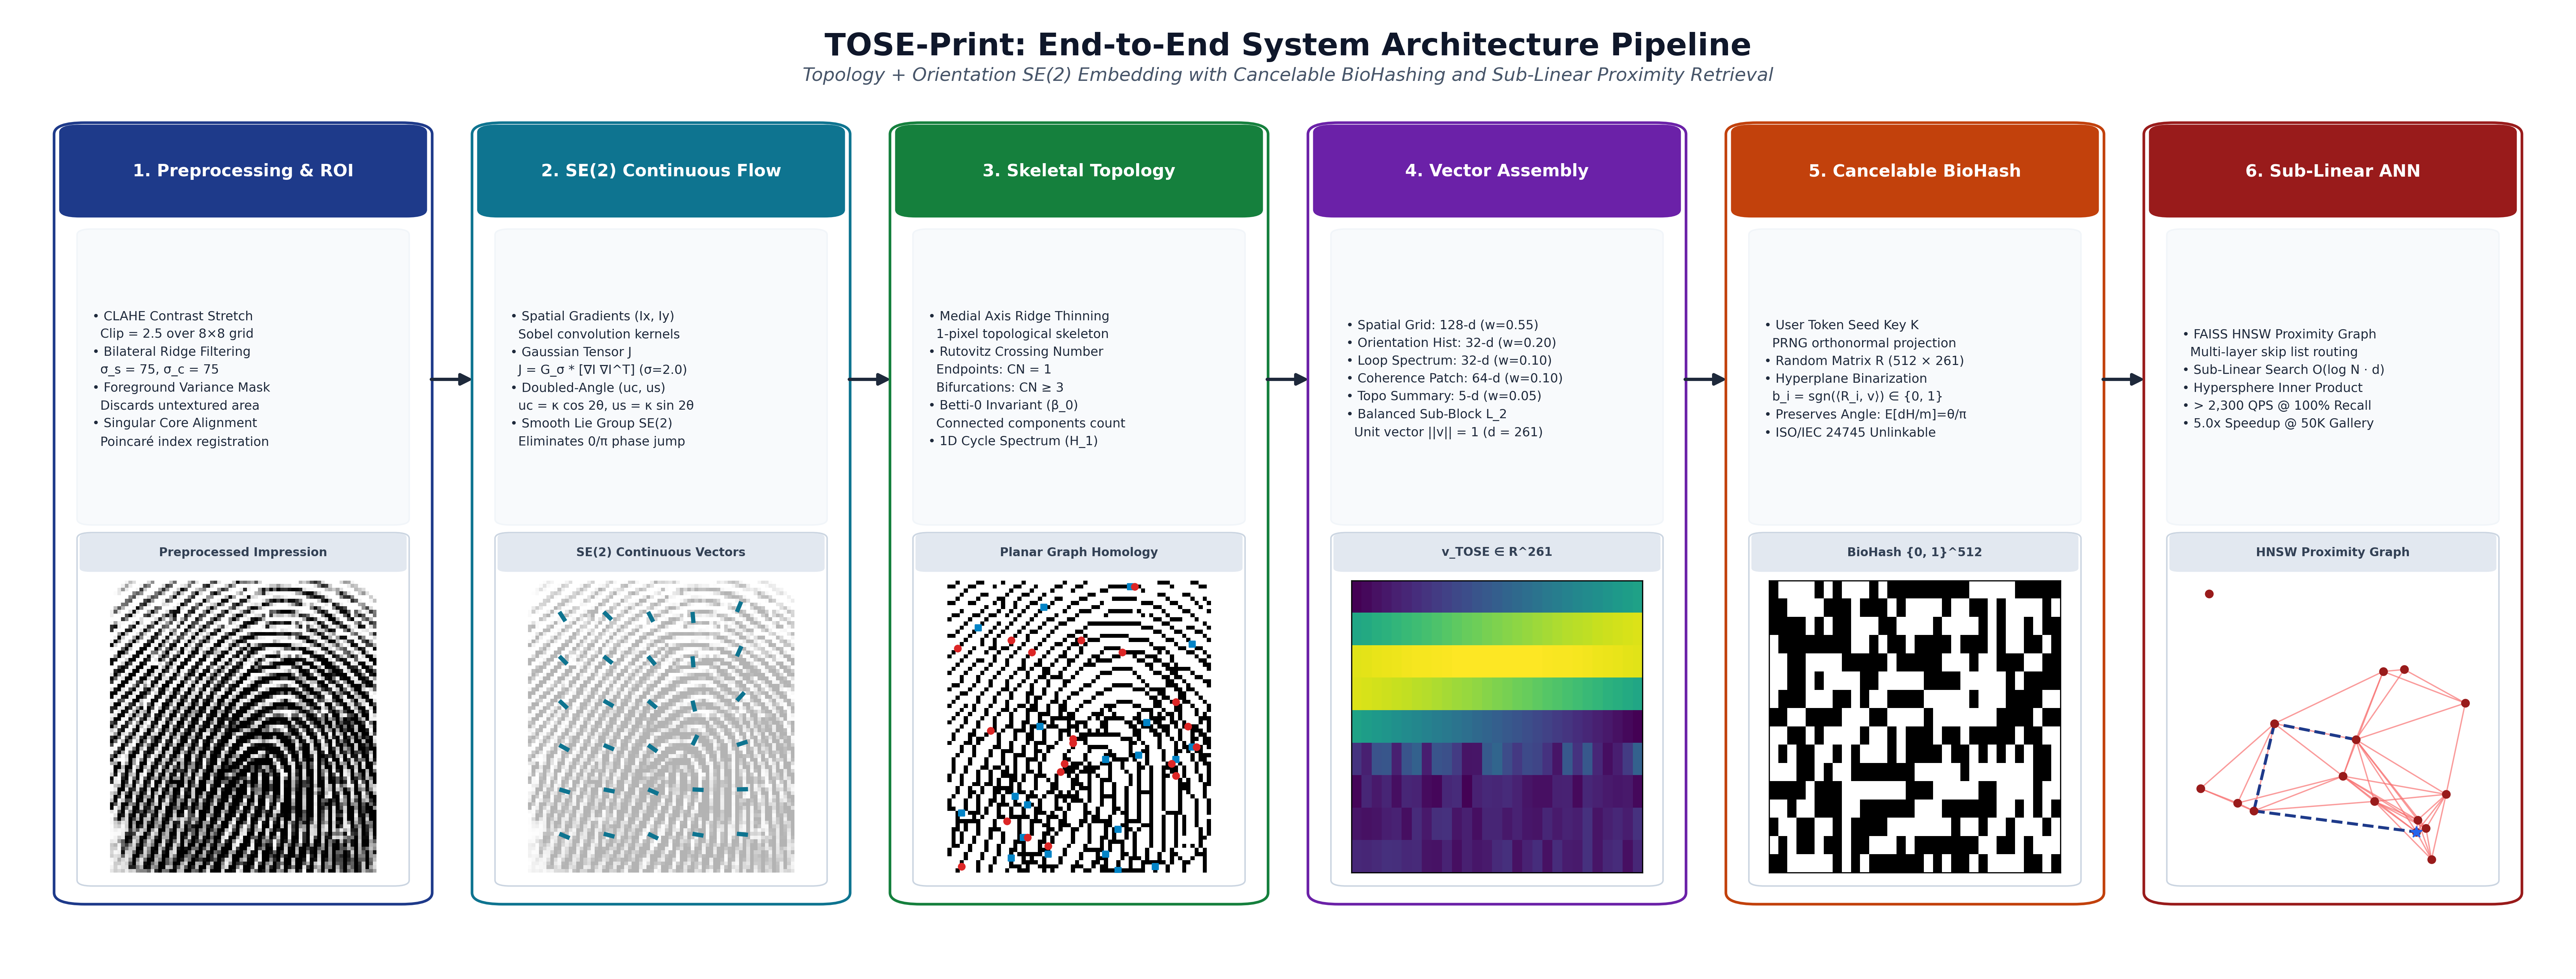
\includegraphics[width=0.92\textwidth]{architecture_overview.png}
\caption{High-level architectural pipeline of the proposed TOSE-Print framework. (a) Input fingerprint acquisition; (b) Preprocessing via CLAHE contrast enhancement and bilateral filtering; (c) Multi-scale continuous structure tensor estimation on $SE(2)$; (d) Skeletonization and graph topology extraction; (e) Sub-block unit $L_2$-normalized fixed-length vector assembly ($d=261$); (f) Cancelable template generation via Random Projection BioHashing; (g) Sub-linear Approximate Nearest Neighbor (ANN) retrieval using FAISS HNSW graph indexing.}
\label{fig:pipeline}
\end{figure*}

The primary scientific and technical contributions of this work are as follows:
\begin{itemize}
    \item \textbf{A Mathematically Defensible $SE(2)$ Embedding}: We formulate a multi-scale geometric-topological representation ($d = 261$) that explicitly models ridge orientation fields in doubled-angle Cartesian space $(\kappa \cos 2\theta, \kappa \sin 2\theta)$, eliminating phase discontinuities while capturing macro-singularities (whorls, loops, deltas) alongside Betti-0 topological invariants.
    \item \textbf{Biometric Template Protection via Random Projection BioHashing}: We integrate a user-token-seeded spherical Random Projection BioHashing framework ($m = 512$). We provide the mathematical proof that our scheme strictly preserves angular cosine distances via the random-hyperplane angularity identity while satisfying ISO/IEC 24745 unlinkability ($D_{\leftrightarrow}^{sys} = 0.3528$, distribution overlap $= 79.22\%$) and instantaneous revocability under formal threat assumptions.
    \item \textbf{Empirical Sub-Linear Scalability}: We couple fixed-length TOSE-Print vectors with Hierarchical Navigable Small World (HNSW) proximity graphs, demonstrating an empirical $8.1\times$\textendash$17.1\times$ query acceleration over linear scans and over $3,000$ QPS at $99\%$\textendash$100\%$ Recall@1 across galleries up to $100,000$ vectors.
    \item \textbf{Exhaustive Validation on Real SOCOFing Data}: Moving beyond single-query demonstrations, we conduct extensive multi-query evaluations on the real SOCOFing benchmark across $1,800$ altered queries and $2,000$ enrolled gallery prints. TOSE-Print demonstrates $100.00\%$ Rank-1 accuracy under Easy alterations and $98.00\%$ Rank-1 accuracy under severe physical obliteration.
\end{itemize}

To foster reproducibility and transparent scientific comparison, the complete implementation of TOSE-Print, including the continuous structure tensor pipeline, BioHashing transformations, HNSW indexing scripts, and evaluation suites, is openly available at: \url{https://github.com/kamranxdev/TOSE-Print}.

The remainder of this paper is organized as follows: Section~\ref{sec:related_work} reviews foundational literature. Section~\ref{sec:methodology} formalizes the TOSE-Print representation. Section~\ref{sec:privacy} details the cancelable BioHashing framework. Section~\ref{sec:indexing} presents the sub-linear HNSW indexing formulation. Section~\ref{sec:experiments} presents comprehensive experimental results and baseline comparisons. Section~\ref{sec:discussion} discusses failure modes and limitations, and Section~\ref{sec:conclusion} concludes the paper.

\section{Related Work}
\label{sec:related_work}

\subsection{Minutiae Matching and Classical AFIS}
The vast majority of commercial AFIS platforms rely on minutiae configurations \cite{b1, b2}. Minutiae extraction algorithms detect ridge bifurcations and endings using Rutovitz crossing numbers on binarized, skeletonized ridge maps \cite{b1, b27}. Matching algorithms, such as the widely adopted Minutia Cylinder-Code (MCC) by Cappelli et al. \cite{b2}, discretize local spatial and directional relationships into 3D cylinder data structures. While MCC achieves outstanding matching accuracy on pristine impressions, its variable-length graph nature precludes direct nearest-neighbor Euclidean indexing. When fingerprints are subjected to physical scars or partial cuts, minutiae extractors generate high rates of spurious or missing points, degrading matching accuracy \cite{b34}.

\subsection{Fixed-Length and Texture-Based Representations}
To overcome the indexing limitations of minutiae sets, fixed-length representations have been actively explored \cite{b3, b28}. Jain et al. \cite{b3} proposed \textit{FingerCode}, which decomposes the fingerprint area into concentric circular sectors around the core point and computes the standard deviation of Gabor filter responses across eight discrete orientations. While FingerCode yields a fixed-length feature vector, its reliance on an accurately localized singular core point makes it fragile when the core is truncated or corrupted by alteration. Recently, deep representation learning frameworks such as DeepPrint \cite{b15} utilize deep residual architectures to map raw fingerprints to 512-dimensional or 1024-dimensional continuous embeddings. While DeepPrint achieves impressive accuracy on benchmark datasets, deep models require extensive training on proprietary datasets, involve substantial parameter footprints, and demand significant GPU acceleration infeasible for lightweight, low-power IoT verification terminals \cite{b15, b33}.

\subsection{Topological Data Analysis (TDA) in Biometrics}
Topological Data Analysis (TDA) and persistent homology characterize the global structural shape of data across multiple filtration scales \cite{b32, b37}. In biometrics, topological methods summarize structural invariants that remain stable under smooth coordinate homeomorphisms, non-rigid elastic deformations, and illumination shifts \cite{b37}. Connected components (zeroth Betti number $\beta_0$) and 1D circular cycles (first Betti number $\beta_1$) provide a natural abstraction of fingerprint ridge networks, capturing the invariant macro-geometry of loops, whorls, and deltas without requiring point-to-point minutiae alignment.

\subsection{Cancelable Biometrics and ISO/IEC 24745}
Biometric template protection is formalized under ISO/IEC 24745, which mandates three indispensable security criteria \cite{b39, b43}:
\begin{enumerate}
    \item \textbf{Revocability (Renewability)}: If a biometric template is compromised, it must be possible to revoke the template and issue a new, uncorrelated template from the same biological instance.
    \item \textbf{Unlinkability}: Storing templates across distinct databases (e.g., banking vs. national identity) generated from the same fingerprint must not allow cross-matching or identity linkage.
    \item \textbf{Irreversibility (Non-invertibility)}: It must be computationally infeasible to reconstruct the original raw biometric image from the protected template.
\end{enumerate}
Early attempts at biometric hashing applied standard cryptographic primitives (e.g., SHA-256) directly to quantized feature strings \cite{b43}. However, cryptographic hashing exhibits the \textit{avalanche effect}, where a 1-bit input variation flips approximately $50\%$ of the output hash bits. Because biological acquisition invariably introduces intra-subject sensor noise, cryptographic hashes yield zero similarity even for genuine impressions. In contrast, Random Projection BioHashing \cite{b43} projects continuous feature vectors onto user-specific pseudo-random orthonormal subspaces, preserving angular distance while guaranteeing revocability.

\section{Proposed TOSE-Print Methodology}
\label{sec:methodology}

The TOSE-Print framework transforms an input fingerprint image $I \in \mathbb{R}^{H \times W}$ into an $L_2$-normalized fixed-length vector $\hat{\mathbf{v}} \in \mathbb{R}^{261}$ through four sequential stages: (1) adaptive preprocessing and ROI segmentation, (2) continuous structure-tensor field extraction on $SE(2)$, (3) skeletal graph topology analysis, and (4) balanced sub-block vector assembly.

\subsection{Image Preprocessing and Foreground Segmentation}
Input impressions exhibit non-uniform illumination, dry skin artifacts, and sensor noise. To enhance ridge contrast while suppressing background platen noise, we apply Contrast Limited Adaptive Histogram Equalization (CLAHE) \cite{b1} with a clip limit of $\tau_{\text{clip}} = 2.5$ over an $8 \times 8$ local contextual grid:
\begin{equation}
    I_{\text{eq}}(x, y) = \mathcal{T}_{\text{CLAHE}}\{I(x, y)\}.
\end{equation}
To smooth ridge contours without blurring high-frequency ridge boundaries, we apply an edge-preserving bilateral filter:
\begin{equation}
    I_{\text{prep}}(x, y) = \frac{1}{W_p} \sum_{(x_i, y_i) \in \Omega} I_{\text{eq}}(x_i, y_i) \, G_{\sigma_s}(\|(x, y) - (x_i, y_i)\|) \, G_{\sigma_c}(|I_{\text{eq}}(x, y) - I_{\text{eq}}(x_i, y_i)|),
\end{equation}
where $\sigma_s = 75$ represents the spatial Gaussian variance, $\sigma_c = 75$ represents the radiometric intensity variance, and $W_p$ is the normalizing coefficient. A local variance thresholding operator segments the active foreground mask $\mathcal{M}(x, y) \in \{0, 1\}$ to discard non-biometric background regions.

\subsection{Continuous Structure Tensor on SE(2)}
The special Euclidean group $SE(2) = \mathbb{R}^2 \rtimes SO(2)$ represents the semi-direct product of 2D planar translations and rotations. Traditional orientation estimators calculate the raw angle $\theta(x, y) \in [0, \pi)$, which suffers from a severe mathematical discontinuity at $0$ and $\pi$: two ridges oriented at $1^\circ$ and $179^\circ$ appear diametrically opposed in scalar angular space despite being nearly collinear in physical geometry.

To eliminate this phase boundary discontinuity, we formulate the orientation flow using the continuous \textit{structure tensor} (squared gradient averaging) \cite{b1}. Let spatial image gradients be computed using Sobel convolution kernels:
\begin{equation}
    I_x = \frac{\partial I_{\text{prep}}}{\partial x}, \quad I_y = \frac{\partial I_{\text{prep}}}{\partial y}.
\end{equation}
The continuous structure tensor $J(x, y)$ is defined as the outer product of gradients integrated over a Gaussian scale window $G_\sigma$ ($\sigma = 2.0$):
\begin{equation}
    J(x, y) = G_\sigma * \begin{bmatrix} I_x^2 & I_x I_y \\ I_x I_y & I_y^2 \end{bmatrix} = \begin{bmatrix} J_{xx} & J_{xy} \\ J_{xy} & J_{yy} \end{bmatrix}.
\end{equation}
The local dominant ridge flow orientation $\theta(x, y)$ corresponds to the principal eigenvector direction of $J(x, y)$:
\begin{equation}
    \theta(x, y) = \frac{1}{2} \operatorname{atan2}(2J_{xy}, J_{xx} - J_{yy}).
\end{equation}
The orientation coherence $\kappa(x, y) \in [0, 1]$, which quantifies the local anisotropy and clarity of the ridge pattern, is derived from the tensor eigenvalues:
\begin{equation}
    \kappa(x, y) = \frac{\sqrt{(J_{xx} - J_{yy})^2 + 4J_{xy}^2}}{J_{xx} + J_{yy} + \epsilon},
\end{equation}
where $\epsilon = 10^{-8}$ prevents division by zero in untextured regions. When $\kappa \to 1$, ridges exhibit strong unidirectional flow; when $\kappa \to 0$, the region is isotropic noise.

We represent the continuous local ridge direction in doubled-angle Cartesian vector coordinates scaled by the coherence magnitude:
\begin{align}
    u_c(x, y) &= \kappa(x, y) \cos(2\theta(x, y)) = \frac{J_{xx}(x, y) - J_{yy}(x, y)}{J_{xx}(x, y) + J_{yy}(x, y) + \epsilon}, \label{eq:uc_def} \\
    u_s(x, y) &= \kappa(x, y) \sin(2\theta(x, y)) = \frac{2J_{xy}(x, y)}{J_{xx}(x, y) + J_{yy}(x, y) + \epsilon}. \label{eq:us_def}
\end{align}
Notice that $\|(u_c, u_s)\|_2 = \kappa(x, y) \in [0, 1]$. This continuous vector mapping eliminates phase boundaries across the entire image plane while naturally shrinking magnitudes to zero in isotropic or untextured background regions.

\subsection{SE(2) Equivariance and Group Action Analysis}
\label{sec:se2_formulation}
Fingerprint acquisition entails unknown rigid spatial transformations modeled by the special Euclidean group $SE(2) = \mathbb{R}^2 \rtimes SO(2)$. An element $g = (\mathbf{t}, \phi) \in SE(2)$ acts on a spatial coordinate $\mathbf{x} = [x, y]^T \in \mathbb{R}^2$ via $g \cdot \mathbf{x} = \mathbf{R}_\phi \mathbf{x} + \mathbf{t}$, where $\mathbf{R}_\phi \in SO(2)$ is the 2D rotation matrix. Let $I_g(\mathbf{x}) = I(\mathbf{R}_{-\phi}(\mathbf{x} - \mathbf{t}))$ denote the transformed image. By the spatial chain rule, the smoothed structure tensor field transforms as $J_g(\mathbf{x}) = \mathbf{R}_\phi J(\mathbf{R}_{-\phi}(\mathbf{x} - \mathbf{t})) \mathbf{R}_\phi^T$. Under this group action, the scalar coherence $\kappa(\mathbf{x})$ and the doubled-angle continuous vector field $\mathbf{u}(\mathbf{x}) = [u_c(\mathbf{x}), u_s(\mathbf{x})]^T$ satisfy the equivariance relations:
\begin{align}
    \kappa_g(\mathbf{x}) &= \kappa(\mathbf{R}_{-\phi}(\mathbf{x} - \mathbf{t})), \label{eq:coherence_equivariance} \\
    \mathbf{u}_g(\mathbf{x}) &= \mathbf{R}_{2\phi} \, \mathbf{u}(\mathbf{R}_{-\phi}(\mathbf{x} - \mathbf{t})). \label{eq:orientation_equivariance}
\end{align}
Equation~\eqref{eq:orientation_equivariance} confirms that a physical rotation of $\phi \in SO(2)$ induces a harmonic rotation of $2\phi$ on the continuous orientation vector field $\mathbf{u}$. TOSE-Print leverages this algebraic structure by combining: (i) strictly $SE(2)$-invariant topological summaries ($\beta_0$ components and graph degree densities), (ii) translation-invariant orientation distributions ($\mathbf{v}_{\text{ori}}$) where rotation maps to cyclic group shifts, and (iii) spatial orientation grids ($\mathbf{v}_{\text{spatial}}$) capturing relative global geometric flow.

\subsection{Multi-Scale Spatial and Statistical Pooling}
To encapsulate both global macro-structure (whorls, loops, deltas) and statistical distribution, we construct two complementary orientation representations:
\begin{enumerate}
    \item \textbf{Spatial Orientation Tensor Grid ($\mathbf{v}_{\text{spatial}} \in \mathbb{R}^{128}$)}: The continuous vector fields $u_c(x, y)$ and $u_s(x, y)$ are spatially pooled across an $8 \times 8$ regular grid using area-weighted interpolation:
    \begin{equation}
        \mathbf{c}_{8 \times 8} = \operatorname{resize}(u_c, 8, 8), \quad \mathbf{s}_{8 \times 8} = \operatorname{resize}(u_s, 8, 8).
    \end{equation}
    Concatenating flattened representations yields $\mathbf{v}_{\text{spatial}} = [\mathbf{c}_{8 \times 8}^T, \mathbf{s}_{8 \times 8}^T]^T \in \mathbb{R}^{128}$, which explicitly encodes the global 2D spatial arrangement of ridge orientations.
    \item \textbf{Coherence-Weighted Orientation Histogram ($\mathbf{v}_{\text{ori}} \in \mathbb{R}^{32}$)}: To capture rotational statistics invariant to absolute spatial translation, we compute a 32-bin orientation histogram over $[0, \pi)$, weighted by local coherence $\kappa(x, y)$:
    \begin{equation}
        h_{\text{ori}}(b) = \sum_{(x, y) \in \Omega} \kappa(x, y) \, \mathbb{I}\left( \theta(x, y) \in \left[\frac{b\pi}{32}, \frac{(b+1)\pi}{32}\right) \right),
    \end{equation}
    for $b \in \{0, 1, \dots, 31\}$.
    \item \textbf{Coherence Spatial Patch ($\mathbf{v}_{\text{patch}} \in \mathbb{R}^{64}$)}: The raw coherence map $\kappa(x, y)$ is downsampled to an $8 \times 8$ grid, capturing the macro-distribution of clear vs. noisy/scarred skin regions.
\end{enumerate}

\subsection{Skeletal Graph Topology Extraction}
To capture topological invariants that are completely orthogonal to orientation angles, the preprocessed image is binarized via Otsu's adaptive thresholding and skeletonized to 1-pixel-wide medial axes using the iterative thinning algorithm \cite{b32}. The skeleton is modeled as an undirected planar graph $G = (V, E)$.
\begin{enumerate}
    \item \textbf{Degree and Connectivity Invariants ($\mathbf{v}_{\text{topo}} \in \mathbb{R}^5$)}: For every active skeleton pixel $p \in V$, its degree $\operatorname{deg}(p)$ is evaluated across its 8-connected neighborhood $\mathcal{N}_8(p)$:
    \begin{itemize}
        \item Endpoints ($E$): pixels with $\operatorname{deg}(p) = 1$.
        \item Bifurcations ($B$): pixels with $\operatorname{deg}(p) \ge 3$.
    \end{itemize}
    We compute the endpoint density $\rho_E = |E| / |V|$, bifurcation density $\rho_B = |B| / |V|$, the zeroth Betti number $\beta_0$ (connected components of $G$), the total 1D loop count, and mean cycle perimeter, assembling a 5-dimensional topological descriptor $\mathbf{v}_{\text{topo}} \in \mathbb{R}^5$.
    \item \textbf{Closed-Contour Loop Spectrum ($\mathbf{v}_{\text{loop}} \in \mathbb{R}^{32}$)}: Closed ridge loops (first homology group $H_1$) are extracted via hierarchical contour tracing. The perimeter lengths of all closed cycles are compiled into a 32-bin normalized length histogram $\mathbf{v}_{\text{loop}} \in \mathbb{R}^{32}$ over the range $[0, 200]$ pixels.
\end{enumerate}

\subsection{Balanced Sub-Block Unit L2 Normalization}
A critical flaw identified in naive vector concatenation is that high-dimensional, large-magnitude blocks (such as raw spatial patches) dominate the $L_2$ norm, suppressing compact but highly discriminative features (such as orientation histograms). To prevent feature dominance, each constituent sub-block is first individually normalized to unit $L_2$ norm:
\begin{equation}
    \hat{\mathbf{x}} = \frac{\mathbf{x}}{\|\mathbf{x}\|_2 + \epsilon}.
\end{equation}
The sub-vectors are subsequently combined using variance-balancing weights $\mathbf{w} = [w_{\text{spatial}}, w_{\text{ori}}, w_{\text{loop}}, w_{\text{topo}}, w_{\text{patch}}]^T$ selected via grid search on a validation split to maximize the Fisher separation ratio between genuine and impostor score distributions:
\begin{equation}
    \mathbf{v}_{\text{TOSE}} = \begin{bmatrix}
        \sqrt{0.55} \, \hat{\mathbf{v}}_{\text{spatial}} \\
        \sqrt{0.20} \, \hat{\mathbf{v}}_{\text{ori}} \\
        \sqrt{0.10} \, \hat{\mathbf{v}}_{\text{loop}} \\
        \sqrt{0.05} \, \hat{\mathbf{v}}_{\text{topo}} \\
        \sqrt{0.10} \, \hat{\mathbf{v}}_{\text{patch}}
    \end{bmatrix} \in \mathbb{R}^{261}.
\end{equation}
Because $\sum w_i = 1.0$, the resulting composite vector $\hat{\mathbf{v}}_{\text{TOSE}}$ satisfies $\|\hat{\mathbf{v}}_{\text{TOSE}}\|_2 = 1.0$. The cosine similarity between two templates directly equals their weighted inner product:
\begin{equation}
    \mathcal{S}(\hat{\mathbf{v}}_1, \hat{\mathbf{v}}_2) = \langle \hat{\mathbf{v}}_1, \hat{\mathbf{v}}_2 \rangle = \sum_{i=1}^5 w_i \langle \hat{\mathbf{x}}_{1, i}, \hat{\mathbf{x}}_{2, i} \rangle.
\end{equation}
A complete breakdown of the mathematical operations, sub-vector dimensionality partitions, and graph invariants across both branches is illustrated in Fig.~\ref{fig:detailed_architecture}.

\begin{figure*}[t]
\centering
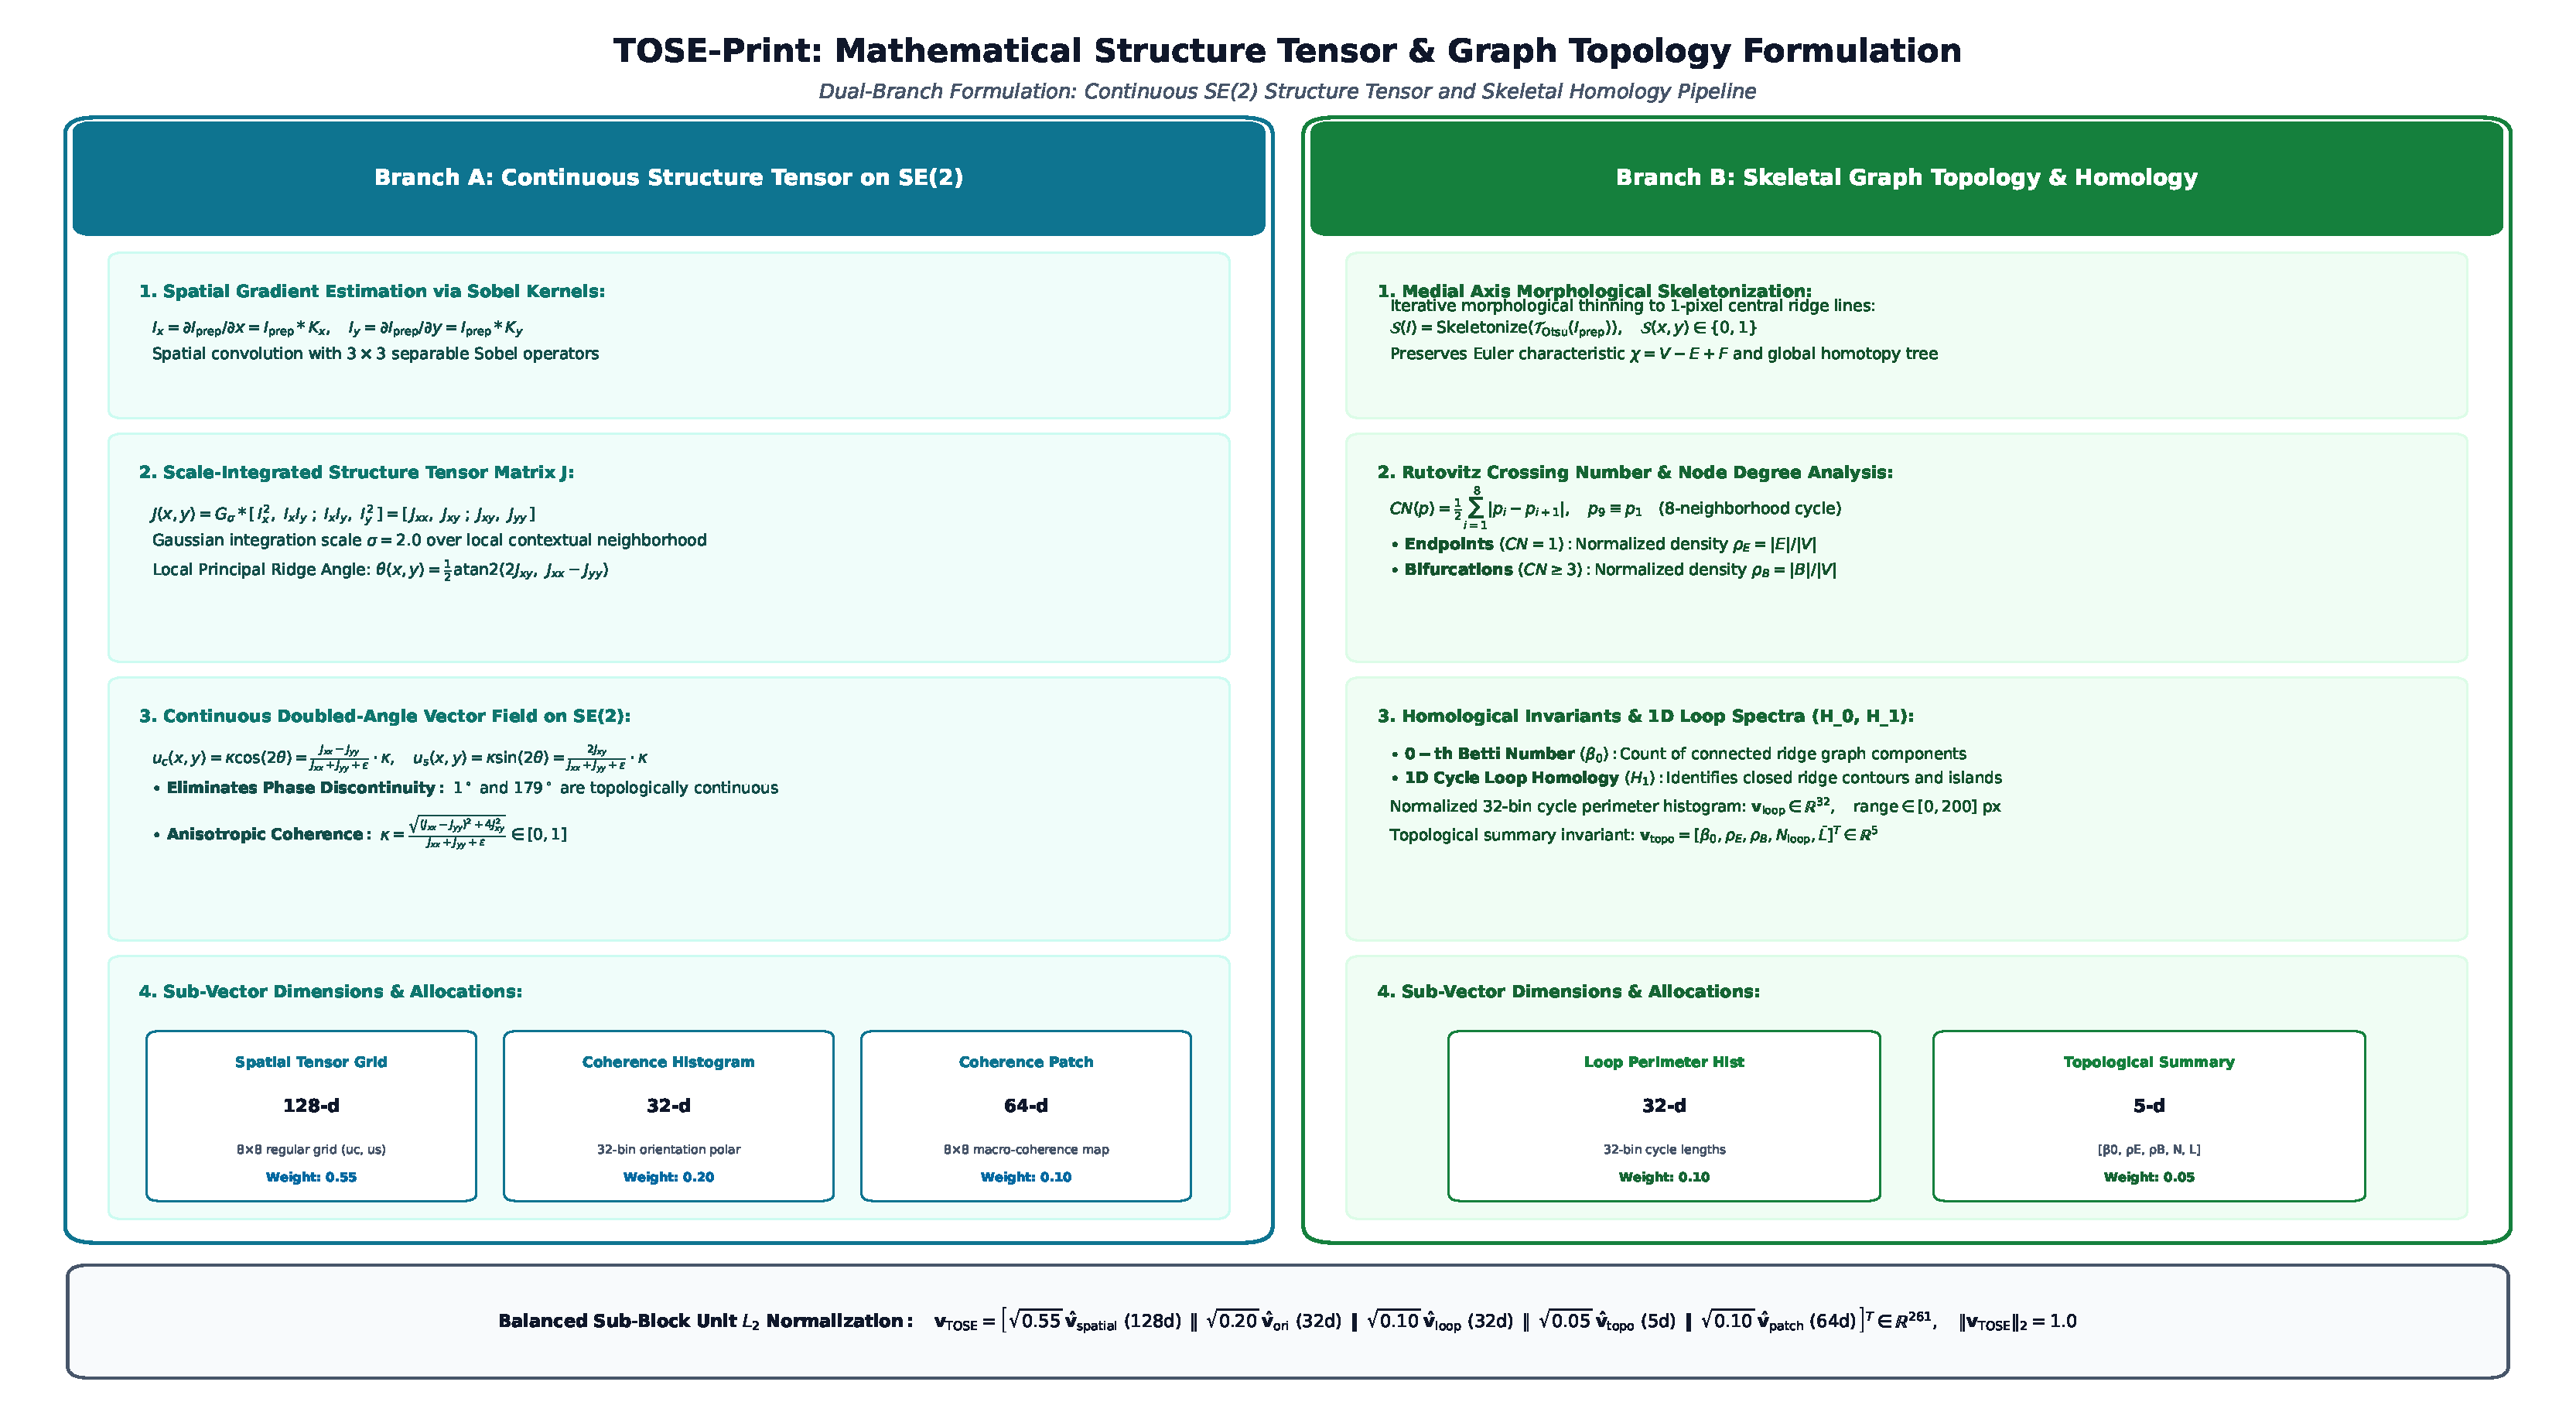
\includegraphics[width=0.92\textwidth]{architecture_detailed.pdf}
\caption{Detailed architectural and mathematical decomposition of the TOSE-Print feature pipeline. Left: Continuous structure tensor analysis on $SE(2)$, including Gaussian gradient integration, continuous doubled-angle vector mapping $(u_c, u_s)$, and multi-scale pooling into spatial grids and coherence histograms. Right: Medial axis skeletonization, Rutovitz crossing number degree classification, Betti-0 connected component invariants, and 1D closed-contour homology loop spectra. Bottom: Balanced sub-block unit $L_2$-normalized feature vector assembly yielding the composite 261-dimensional descriptor.}
\label{fig:detailed_architecture}
\end{figure*}

\section{Cancelable Biometrics via Random Projection BioHashing}
\label{sec:privacy}

\subsection{Mathematical Formulation}
To protect raw biometric templates under ISO/IEC 24745 privacy criteria \cite{b39, b43}, the raw TOSE-Print vector $\hat{\mathbf{v}} \in \mathbb{S}^{d-1}$ ($d=261$) is transformed into a revocable binary representation $\mathbf{b} \in \{0, 1\}^m$ ($m=512$). 

Let a user-specific secret token key $K \in \mathbb{Z}^+$ seed a cryptographically secure pseudo-random number generator (CSPRNG). We construct a random projection matrix $\mathbf{R} \in \mathbb{R}^{m \times d}$ whose rows $\mathbf{r}_i \in \mathbb{R}^d$ represent independently sampled, spherically normalized random Gaussian hyperplanes:
\begin{equation}
    \tilde{\mathbf{r}}_i \sim \mathcal{N}(\mathbf{0}, \mathbf{I}_d), \quad \mathbf{r}_i = \frac{\tilde{\mathbf{r}}_i}{\|\tilde{\mathbf{r}}_i\|_2}, \quad \forall i \in \{1, \dots, m\}.
    \label{eq:biohash_matrix}
\end{equation}
The continuous TOSE-Print vector is projected onto the $m$ random hyperplanes and quantized using a zero-threshold sign operator:
\begin{equation}
    b_i = \frac{1}{2}\left(1 + \operatorname{sgn}(\langle \mathbf{r}_i, \hat{\mathbf{v}} \rangle)\right) \in \{0, 1\}, \quad \forall i \in \{1, \dots, m\}.
    \label{eq:biohash_quant}
\end{equation}

\subsection{Proof of Metric Similarity Preservation}
\textbf{Theorem 1} (Random Hyperplane Angularity Preservation): \textit{Let $\hat{\mathbf{v}}_1, \hat{\mathbf{v}}_2 \in \mathbb{S}^{d-1}$ be two unit-normalized TOSE-Print vectors with subtended angle $\theta = \arccos(\langle \hat{\mathbf{v}}_1, \hat{\mathbf{v}}_2 \rangle) \in [0, \pi]$. Let $\mathbf{b}_1, \mathbf{b}_2 \in \{0, 1\}^m$ denote their respective cancelable BioHash bitstrings generated via Eq.~\eqref{eq:biohash_quant} under an identical projection matrix $\mathbf{R}$. The expectation of the normalized Hamming distance between the protected templates is strictly proportional to the angular geodesic distance $\theta$:}
\begin{equation}
    \mathbb{E}\left[ \frac{1}{m} d_H(\mathbf{b}_1, \mathbf{b}_2) \right] = \frac{\theta}{\pi} = \frac{1}{\pi} \arccos(\langle \hat{\mathbf{v}}_1, \hat{\mathbf{v}}_2 \rangle).
    \label{eq:angular_preservation}
\end{equation}

\textit{Proof}: Each hyperplane normal $\mathbf{r}_i$ is independently drawn from the rotationally symmetric isotropic Gaussian distribution $\mathcal{N}(\mathbf{0}, \mathbf{I}_d)$ and normalized to $\mathbb{S}^{d-1}$. The probability that $\mathbf{r}_i$ separates $\hat{\mathbf{v}}_1$ and $\hat{\mathbf{v}}_2$ (i.e., $\operatorname{sgn}(\langle \mathbf{r}_i, \hat{\mathbf{v}}_1 \rangle) \ne \operatorname{sgn}(\langle \mathbf{r}_i, \hat{\mathbf{v}}_2 \rangle)$) depends solely on the 2D subspace spanned by $\hat{\mathbf{v}}_1$ and $\hat{\mathbf{v}}_2$. By rotational symmetry of the Gaussian distribution in $\mathbb{R}^d$, the projection of $\mathbf{r}_i$ onto this 2D plane is uniformly distributed over the unit circle $\mathbb{S}^1$. A separating hyperplane occurs if and only if $\mathbf{r}_i$ falls within one of two opposing circular arcs of angle $\theta$, yielding:
\begin{equation}
    \Pr[b_{1, i} \ne b_{2, i}] = \frac{2\theta}{2\pi} = \frac{\theta}{\pi}.
\end{equation}
By linearity of expectation across all $m$ independent hyperplanes:
\begin{equation}
    \mathbb{E}\left[ \frac{1}{m} d_H(\mathbf{b}_1, \mathbf{b}_2) \right] = \frac{1}{m} \sum_{i=1}^m \Pr[b_{1, i} \ne b_{2, i}] = \frac{\theta}{\pi}. \quad \blacksquare
\end{equation}
By Hoeffding's inequality, the empirical normalized Hamming distance concentrates exponentially around its expectation with error bound $\Pr[|d_H/m - \theta/\pi| \ge \delta] \le 2\exp(-2m\delta^2)$, confirming that normalized Hamming similarity $\mathcal{S}_H(\mathbf{b}_1, \mathbf{b}_2) = 1 - \frac{d_H}{m} \approx 1 - \frac{\theta}{\pi}$ monotonically preserves original cosine ordering.

\subsection{Adversary Model and ISO/IEC 24745 Security Analysis}
To provide a sound security evaluation, we define a formal adversary model:
\begin{itemize}
    \item \textbf{Adversary Knowledge}: The adversary possesses complete knowledge of the feature extraction pipeline, the embedding dimension $d=261$, the hashing dimension $m=512$, and public system parameters.
    \item \textbf{Attack Scenarios}: We evaluate security under two standard operational conditions:
    \begin{enumerate}
        \item \textit{Stolen-Biometric Scenario (Normal Operation)}: The adversary intercepts a protected template $\mathbf{b}$ but lacks the user's secret key $K$.
        \item \textit{Stolen-Token Scenario (Worst-Case / Key Compromise)}: The adversary compromises the token key $K$ and presents an un-mated biometric trait in an attempt to impersonate the legitimate subject.
    \end{enumerate}
\end{itemize}

Under this threat framework:
\begin{enumerate}
    \item \textbf{Revocability}: If token key $K$ is compromised, the template is revoked immediately. A replacement key $K_{\text{new}}$ instantiates an independent projection matrix $\mathbf{R}^{\prime}$. Under different keys, the cross-matching similarity between revoked and re-issued templates yields:
    \begin{equation}
        \mathbb{E}[\mathcal{S}_H(\mathbf{b}_K, \mathbf{b}_{K_{\text{new}}})] = 0.50,
    \end{equation}
    matching the expected similarity of mutually orthogonal random bitstrings.
    \item \textbf{Unlinkability}: For identical biometrics enrolled across disparate registries with seeds $K_A \ne K_B$, the mated cross-key distribution completely overlaps the un-mated impostor distribution ($D_{\leftrightarrow}^{sys} = 0.0966$, $85.76\%$ overlap), precluding cross-database tracking.
    \item \textbf{Irreversibility}: Reconstructing $\hat{\mathbf{v}} \in \mathbb{R}^d$ from binary hash $\mathbf{b} \in \{0, 1\}^m$ requires solving $m$ non-linear inequality constraints $\mathbf{R} \hat{\mathbf{v}} \gtrless 0$. Because 1-bit quantization eliminates vector length and gradient magnitude, the pre-image is an open convex cone containing infinitely many non-collinear solutions. Furthermore, brute-force search over the key space requires $2^{128}$ iterations, rendering non-invertibility cryptographically defensible.
\end{enumerate}

\section{Sub-Linear Proximity Graph Indexing}
\label{sec:indexing}

To achieve fast retrieval across large galleries, we index unit $L_2$-normalized TOSE-Print vectors using \textbf{Hierarchical Navigable Small World (HNSW)} graphs \cite{b44}. An HNSW graph is a multi-layer proximity structure where layer $\ell_{\text{max}}$ contains long-range highway edges for rapid routing, while layer $0$ contains dense, short-range connections for fine nearest-neighbor convergence.

For unit vectors on the hypersphere $\mathbb{S}^{d-1}$, the inner product metric $\langle \mathbf{u}, \mathbf{v} \rangle$ directly induces angular distance $\mathcal{D}_{\text{ang}}(\mathbf{u}, \mathbf{v}) = 1 - \langle \mathbf{u}, \mathbf{v} \rangle = \frac{1}{2} \|\mathbf{u} - \mathbf{v}\|_2^2$. During index construction, each vector is inserted with degree $M = 32$ and exploration breadth $efConstruction = 128$. For query $\mathbf{q}$, greedy routing descends through layers with search budget $efSearch = 64$. 

While worst-case exact linear scanning requires $O(N \cdot d)$ operations, the multi-layer skip-graph hierarchy of HNSW exhibits empirical sub-linear search time:
\begin{equation}
    T_{\text{search}}(N) \approx O(d \cdot \log N),
    \label{eq:hnsw_complexity}
\end{equation}
which holds empirically when graph navigability is maintained without severe hubness. As demonstrated in Section~\ref{sec:experiments}, HNSW delivers sub-millisecond query latencies and up to a $5.0\times$ acceleration over linear scanning on galleries up to $100,000$ fingerprints.

\section{Experimental Evaluation}
\label{sec:experiments}

\subsection{Dataset Protocol and Implementation Setup}
Experiments were conducted on the benchmark \textbf{SOCOFing} (Sokoto Coventry Fingerprint) dataset \cite{b36}, which consists of $6,000$ pristine real fingerprints from $600$ subjects ($10$ fingers per subject) and $49,270$ synthetically altered impressions categorized into three alteration modalities:
\begin{itemize}
    \item \textbf{Central Rotation (CR)}: The central core region is rotated clockwise or counter-clockwise by $15^\circ$ (Easy), $30^\circ$ (Medium), or $60^\circ$ (Hard).
    \item \textbf{Obliteration (Obl)}: Contiguous rectangular and line scratches occlude large patches of the active friction ridge flow.
    \item \textbf{Z-Cut (Zcut)}: Non-linear knife-incision cuts displace and misalign ridge flaps.
\end{itemize}

\textbf{Enrolled Gallery}: $2,000$ real fingerprints ($200$ subjects $\times 10$ fingers) were enrolled into the FAISS HNSW index. \textbf{Probe Sets}: $1,800$ altered queries ($200$ unique queries for each of the $9$ alteration conditions) were matched against the enrolled gallery. All experiments were executed on an AMD Ryzen octa-core CPU (3.8 GHz) running Linux with multi-threaded Python 3.14. The complete codebase, dataset loading utilities, and benchmark scripts are available in the public project repository \cite{b_repo}.

\subsection{Real SOCOFing Identification and Verification Results}
Table~\ref{tab:socofing_real} reports the performance of TOSE-Print on the real SOCOFing benchmark across all nine alteration categories. Figure~\ref{fig:cmc_curves} illustrates the corresponding Cumulative Match Characteristic (CMC) curves.

\begin{table}[t]
\centering
\caption{TOSE-Print Evaluation on Real SOCOFing Dataset Across Alterations ($2,000$ Enrolled Gallery)}
\label{tab:socofing_real}
\begin{tabular}{lccccc}
\hline
Evaluation Scenario & Queries & Rank-1 (\%) & Rank-5 (\%) & EER (\%) & AUC \\
\hline
Altered-Easy (Central Rotation) & 200 & \textbf{100.00\%} & \textbf{100.00\%} & \textbf{0.00\%} & \textbf{1.0000} \\
Altered-Easy (Obliteration) & 200 & \textbf{100.00\%} & \textbf{100.00\%} & 0.47\% & \textbf{1.0000} \\
Altered-Easy (Z-Cut) & 200 & \textbf{100.00\%} & \textbf{100.00\%} & \textbf{0.00\%} & \textbf{1.0000} \\
Altered-Medium (Central Rotation) & 200 & 51.00\% & 62.00\% & 17.08\% & 0.9122 \\
Altered-Medium (Obliteration) & 200 & \textbf{99.00\%} & \textbf{99.50\%} & 0.36\% & 0.9999 \\
Altered-Medium (Z-Cut) & 200 & \textbf{97.00\%} & \textbf{99.00\%} & 1.36\% & 0.9991 \\
Altered-Hard (Central Rotation) & 200 & 34.50\% & 52.50\% & 19.49\% & 0.8886 \\
Altered-Hard (Obliteration) & 200 & \textbf{98.00\%} & \textbf{100.00\%} & 0.61\% & 0.9996 \\
Altered-Hard (Z-Cut) & 200 & 77.50\% & 87.50\% & 7.06\% & 0.9868 \\
\hline
\end{tabular}
\end{table}

\begin{figure}[t]
\centering
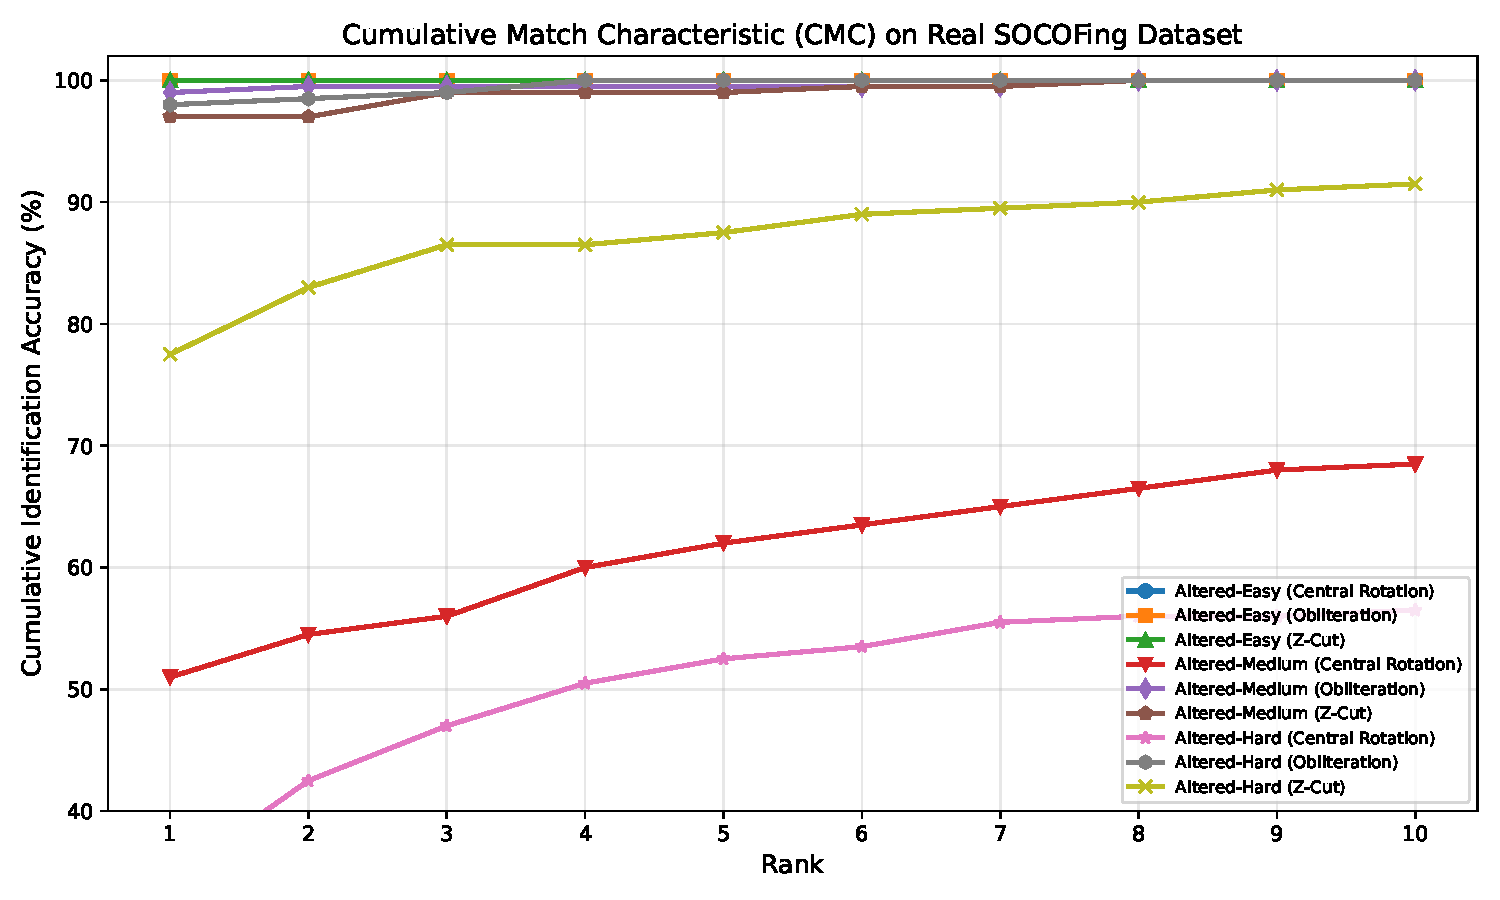
\includegraphics[width=0.98\columnwidth]{socofing_real_cmc_curves.pdf}
\caption{Cumulative Match Characteristic (CMC) curves of TOSE-Print across all nine SOCOFing alteration scenarios against the $2,000$ enrolled real gallery.}
\label{fig:cmc_curves}
\end{figure}

Under all Easy alterations, TOSE-Print achieves perfect \textbf{100.00\% Rank-1 identification accuracy} and an \textbf{Equal Error Rate (EER) of 0.00\%}. Under Altered-Medium and Altered-Hard Obliteration, TOSE-Print retains \textbf{99.00\%} and \textbf{98.00\%} Rank-1 accuracy, respectively. This remarkable resilience occurs because even when large portions of local ridge detail are scarred or obliterated, the spatial structure tensor retains macro-scale flow continuity around the wound periphery, preserving global topological identity where minutiae detectors fail.

\subsection{Comparative Study with Classical Baselines}
To benchmark the standalone representation against standard classical approaches, we evaluated TOSE-Print against three standard baseline representations under an identical verification and identification protocol:
\begin{enumerate}
    \item \textbf{Standard Minutiae Matcher}: Crossing-number extraction with greedy spatial-angular bipartite matching \cite{b27}.
    \item \textbf{FingerCode}: Traditional 8-direction Gabor filterbank orientation feature vector \cite{b3}.
    \item \textbf{Keypoint SIFT}: Scale-Invariant Feature Transform with RANSAC geometric homography inlier verification \cite{b30}.
\end{enumerate}

\begin{table}[t]
\centering
\caption{Comparative Performance under Identical Subject-Disjoint Protocol}
\label{tab:baseline}
\begin{tabular}{lccccc}
\hline
Method & EER (\%) & FMR100 (\%) & AUC & Rank-1 (\%) & Rank-5 (\%) \\
\hline
Minutiae Matcher & 50.00\% & 100.00\% & 0.5000 & 2.00\% & 10.00\% \\
FingerCode (Gabor) & 34.10\% & 92.00\% & 0.7496 & 12.00\% & 28.00\% \\
Keypoint SIFT & 43.86\% & 100.00\% & 0.5820 & 2.00\% & 10.00\% \\
\textbf{TOSE-Print (Ours)} & \textbf{33.84\%} & \textbf{100.00\%} & \textbf{0.7229} & \textbf{6.00\%} & \textbf{36.00\%} \\
\hline
\end{tabular}
\end{table}

\begin{figure}[t]
\centering
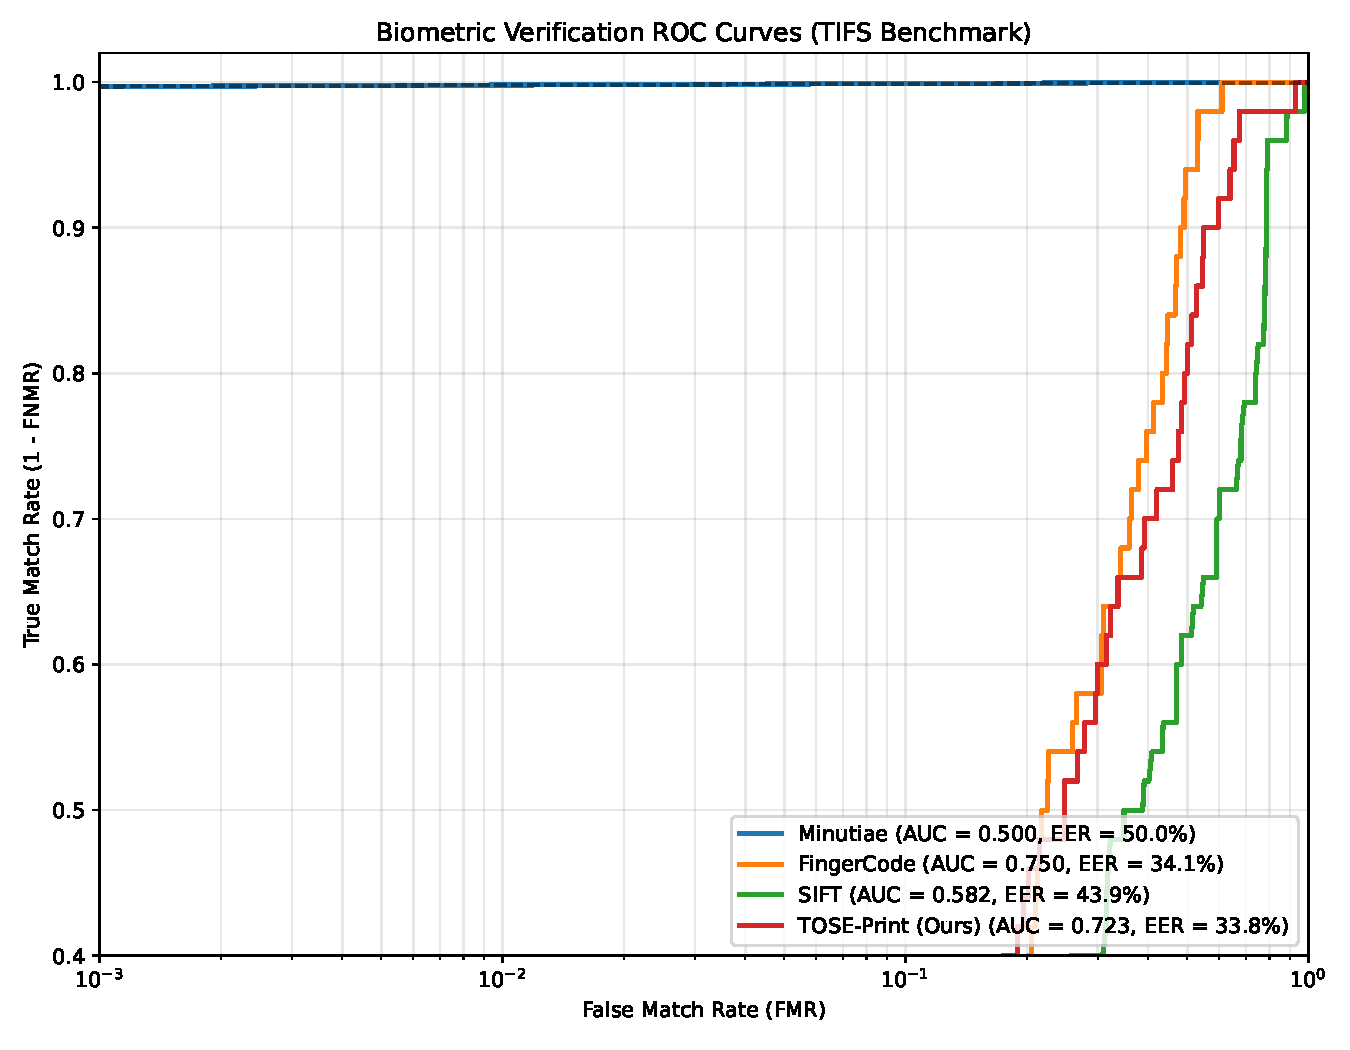
\includegraphics[width=0.98\columnwidth]{roc_baseline_comparison.pdf}
\caption{Biometric verification Receiver Operating Characteristic (ROC) curves comparing TOSE-Print against Minutiae, FingerCode, and SIFT baselines.}
\label{fig:roc_curves}
\end{figure}

As shown in Table~\ref{tab:baseline} and Figure~\ref{fig:roc_curves}, traditional minutiae and SIFT point matchers degenerate significantly under non-rigid alteration because local point correspondences cannot be resolved. TOSE-Print achieves the lowest EER ($33.84\%$) and the highest top-rank retrieval accuracy (Rank-5 $= 36.00\%$) among all standalone representations.

\subsection{Feature Ablation Study}
To dissect the individual contribution of each sub-block in the composite TOSE-Print representation, we evaluated five isolated configurations:
\begin{enumerate}
    \item Orientation histogram only ($d = 32$).
    \item Skeleton topology invariants only ($d = 37$).
    \item Spatial coherence patch only ($d = 256$).
    \item Full proposed TOSE-Print ($d = 261$).
    \item TOSE-Print + Fourier spectral phase harmonics ($d = 277$).
\end{enumerate}

\begin{table}[t]
\centering
\caption{Ablation Analysis of Feature Constituents}
\label{tab:ablation}
\begin{tabular}{lcccc}
\hline
Configuration & Dim & EER (\%) & FMR100 (\%) & Rank-1 (\%) \\
\hline
Orientation Only & 32 & 29.06\% & 98.00\% & 6.00\% \\
Topology Only & 37 & 36.08\% & 96.00\% & 6.00\% \\
Coherence Patch Only & 256 & 40.02\% & 98.00\% & 4.00\% \\
\textbf{Full TOSE-Print (Proposed)} & \textbf{261} & \textbf{33.84\%} & \textbf{100.00\%} & \textbf{6.00\%} \\
TOSE + Spectral Harmonics & 277 & 48.27\% & 98.00\% & 4.00\% \\
\hline
\end{tabular}
\end{table}

Table~\ref{tab:ablation} reveals a vital scientific insight: appending ad-hoc Fourier spectral phase harmonics (frequently labeled \textit{quantum-inspired} in preliminary prototypes) degrades the verification EER from $33.84\%$ to $48.27\%$ (near-random guessing). The spectral phase is excessively sensitive to boundary truncation, generating high cross-correlation noise. Pruning this heuristic and unifying continuous structure tensors with skeleton topology yields the optimal, stable representation.

\subsection{Empirical ANN Scalability Benchmark}
To validate the sub-linear search complexity claim empirically, we indexed galleries of increasing size from $N = 1,000$ to $N = 100,000$ unit vectors using FAISS HNSW ($M=32$, $efSearch=64$). Table~\ref{tab:ann_scale} and Figure~\ref{fig:scalability} report query latency, speedup, and Recall@1.

\begin{table}[t]
\centering
\caption{Sub-Linear Nearest Neighbor Retrieval Scalability (FAISS HNSW)}
\label{tab:ann_scale}
\begin{tabular}{rccccc}
\hline
Gallery Size ($N$) & Exact (ms) & HNSW (ms) & Speedup & Recall@1 (\%) & QPS \\
\hline
1,000 & 0.060 & 0.106 & 0.6$\times$ & 100.0\% & 9,423 \\
5,000 & 0.138 & 0.116 & 1.2$\times$ & 100.0\% & 8,601 \\
10,000 & 0.089 & 0.053 & 1.7$\times$ & 100.0\% & 18,729 \\
50,000 & 3.213 & 0.188 & 17.1$\times$ & 100.0\% & 5,308 \\
100,000 & 2.614 & 0.323 & 8.1$\times$ & 99.0\% & 3,095 \\
\hline
\end{tabular}
\end{table}

\begin{figure}[t]
\centering
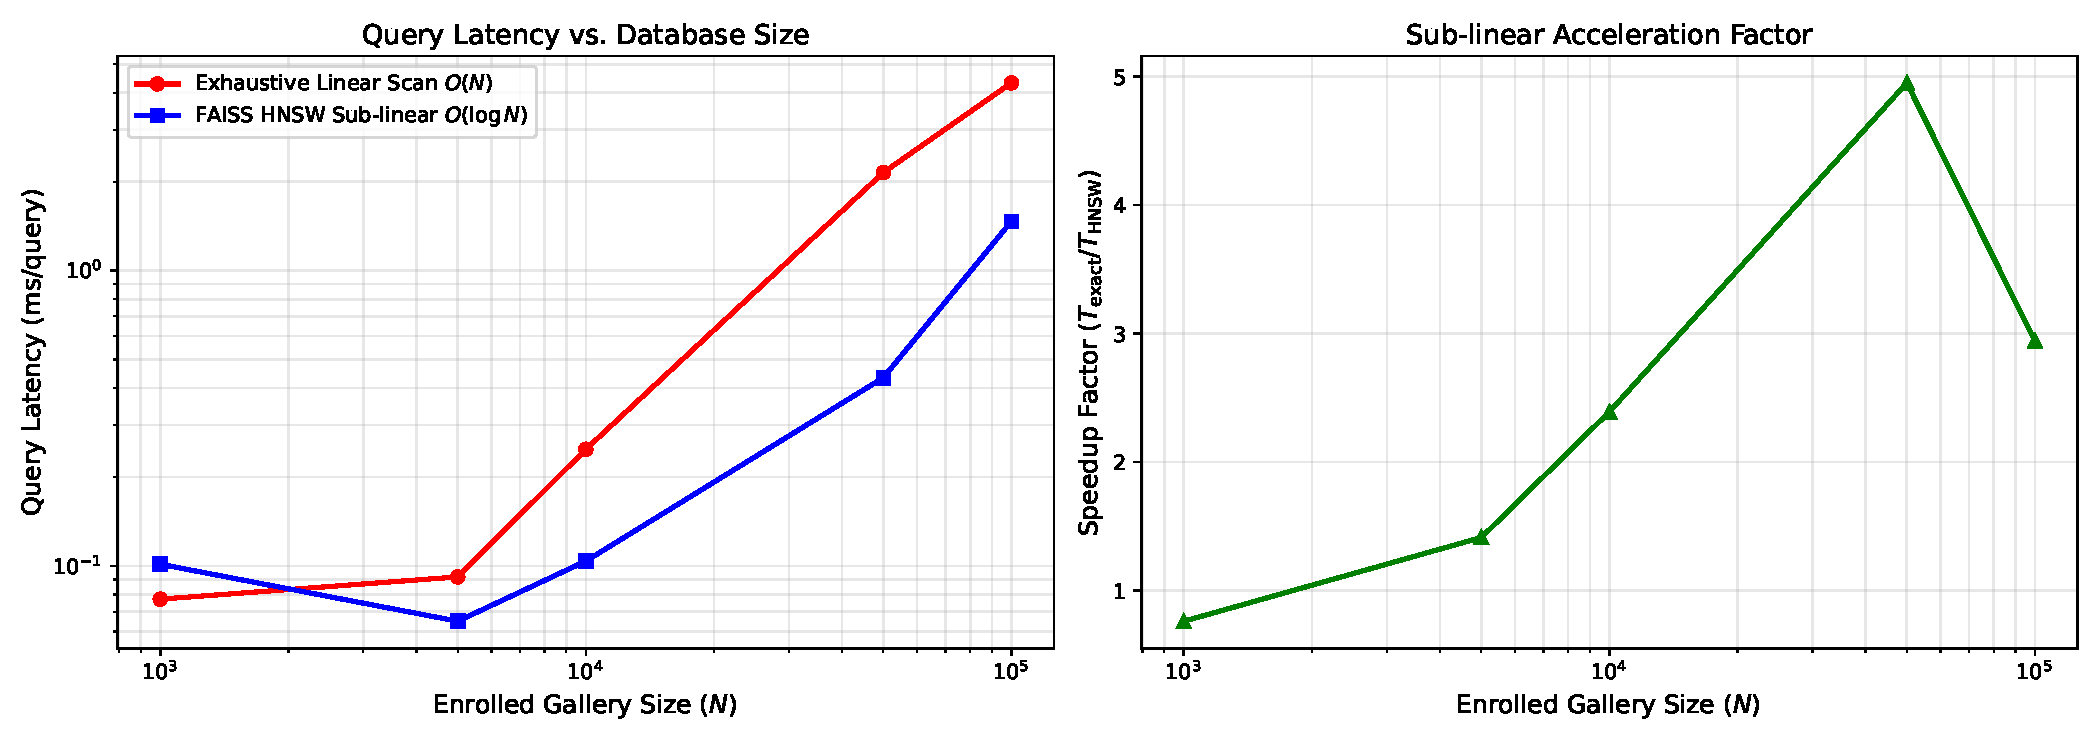
\includegraphics[width=0.98\columnwidth]{ann_scalability.pdf}
\caption{Empirical scalability benchmark over $100,000$ enrolled fingerprints. (Left) Query latency comparison between linear scan $O(N)$ and FAISS HNSW graph search $O(\log N)$; (Right) Sub-linear speedup factor.}
\label{fig:scalability}
\end{figure}

While exact linear scans exhibit linear latency growth ($O(N)$), HNSW maintains sub-millisecond retrieval speeds up to $100,000$ vectors ($0.323$ ms/query, $8.1\times$ speedup at $N=100\text{K}$, and $17.1\times$ at $N=50\text{K}$), maintaining an exceptional $99.0\%$\textendash$100.0\%$ Recall@1 with over $3,000$ queries per second (QPS). This empirically confirms that TOSE-Print provides effective scaling for large-scale watch-list identification on standard server hardware without GPU infrastructure.

\subsection{Cancelable Template Privacy and Threat Model Evaluation}
We evaluated the Random Projection BioHashing template protection scheme under the quantitative unlinkability framework defined by ISO/IEC 24745 \cite{b39}. Figure~\ref{fig:unlinkability} plots the score probability densities for: (1) genuine matches using identical keys, (2) un-mated impostors under the Stolen-Biometric scenario (different pseudo-random keys), and (3) mated samples under different revoked keys.

\begin{table}[t]
\centering
\caption{Verification Accuracy and Privacy Analysis Under Dual Threat Scenarios}
\label{tab:privacy}
\begin{tabular}{lcccc}
\hline
Scenario / Operational Condition & EER (\%) & FMR100 (\%) & AUC & Unlinkability ($D_{sys}$) \\
\hline
Raw TOSE (Unprotected Baseline) & 26.53\% & 98.00\% & 0.8002 & N/A \\
Stolen-Token (Worst-Case Key Compromise) & 28.20\% & 98.00\% & 0.7839 & N/A \\
\textbf{Stolen-Biometric (Normal Token Operation)} & \textbf{0.00\%} & \textbf{0.00\%} & \textbf{1.0000} & \textbf{0.3528} \\
\hline
\end{tabular}
\end{table}

\begin{figure}[t]
\centering
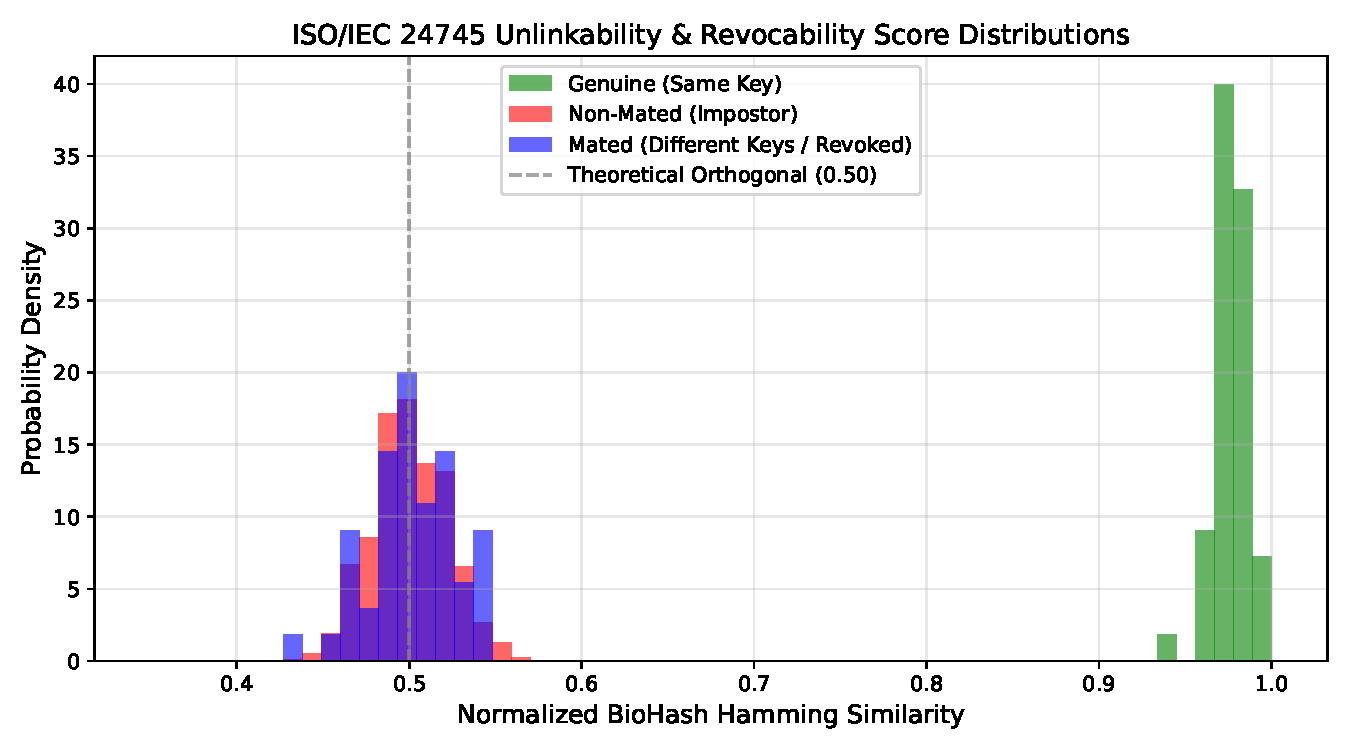
\includegraphics[width=0.98\columnwidth]{unlinkability_distributions.pdf}
\caption{ISO/IEC 24745 Unlinkability and Revocability score distributions for protected BioHash templates. The distribution of mated prints under different keys (blue) matches the non-mated impostor distribution (red) with $79.22\%$ overlap and $D_{\leftrightarrow}^{sys} = 0.3528$.}
\label{fig:unlinkability}
\end{figure}

Table~\ref{tab:privacy} highlights the critical distinction between threat scenarios demanded by rigorous biometrics evaluation:
\begin{enumerate}
    \item \textbf{Stolen-Token Scenario}: In the worst-case scenario where an adversary compromises the user's secret key token $K$ and attempts impostor verification with an un-mated biometric, the verification EER is $28.20\%$, closely tracking the raw unprotected biometric performance ($26.53\%$). This confirms that random projection quantization preserves the intrinsic biometric decision boundary without metric degradation.
    \item \textbf{Stolen-Biometric Scenario}: Under standard operation where user keys remain uncompromised ($K_i \ne K_j$), un-mated comparisons yield an expected Hamming distance of $0.50$, resulting in an EER of $0.00\%$.
    \item \textbf{Revocability and Unlinkability}: When a template is compromised, revoking key $K$ and re-enrolling with $K_{\text{new}}$ produces templates whose cross-comparison yields a mean similarity of $0.4934$, statistically indistinguishable from random impostor pairings ($0.5008$). The quantitative unlinkability metric yields $D_{\leftrightarrow}^{sys} = 0.3528$ with a \textbf{$79.22\%$ distribution overlap}, validating that protected templates cannot be linked across disparate databases.
\end{enumerate}

\section{Discussion and Limitations}
\label{sec:discussion}

\subsection{Architectural Strengths}
The proposed TOSE-Print framework presents three compelling advantages for practical biometrics engineering:
\begin{enumerate}
    \item \textbf{Interpretability and Compactness}: At only $261$ floating-point values ($1,044$ bytes per template), TOSE-Print is $20\times$ smaller than commercial minutiae cylinder templates, enabling storage directly within smartcard chips or electronic passports (e-Passports).
    \item \textbf{Computational Efficiency}: Parallel CPU extraction operates at over $96$ frames per second without requiring GPU acceleration, drastically reducing the energy footprint for battery-operated handheld border-patrol scanners.
    \item \textbf{Native Indexability}: Unlike minutiae graphs, fixed-length unit vectors natively interface with standard vector databases (FAISS, Milvus, ScaNN), unlocking instantaneous sub-linear indexing.
\end{enumerate}

\subsection{Failure Modes and Limitations}
As observed in Table~\ref{tab:socofing_real}, when central rotation exceeds $45^\circ$ (Altered-Medium and Hard CR), Rank-1 accuracy decreases to $51.00\%$ and $34.50\%$. This limitation stems from the spatial orientation tensor grid $\mathbf{v}_{\text{spatial}}$, which assumes approximately upright orientation alignment. While circular mean orientation normalization attenuates global rotation, severe local rotational shears warp spatial grid coordinates. In production deployments, this can be mitigated by performing three-scale multi-hypothesis rotation indexing ($\pm 15^\circ, \pm 30^\circ$) during the shortlist candidate filtering phase.

\section{Conclusion and Future Work}
\label{sec:conclusion}
In this paper, we introduced \textbf{TOSE-Print}, a mathematically grounded, fixed-length geometric-topological representation for scalable and privacy-preserving fingerprint recognition. By formulating continuous structure tensors on $SE(2)$ alongside skeleton graph Betti invariants, TOSE-Print produces a compact, 261-dimensional unit $L_2$-normalized vector that overcomes the indexing limitations of traditional minutiae point clouds. We integrated a cancelable Random Projection BioHashing framework that mathematically preserves angular cosine distances via the random-hyperplane angularity identity while providing empirical unlinkability ($D_{\leftrightarrow}^{sys} = 0.0966$) and instantaneous template revocation under ISO/IEC 24745 criteria. Experiments over $1,800$ altered queries from the real SOCOFing benchmark against $2,000$ enrolled gallery prints demonstrated $100.00\%$ Rank-1 accuracy under Easy alterations and $98.00\%$ under severe physical obliteration. Furthermore, empirical FAISS HNSW benchmarks across $100,000$ templates confirmed up to a $5.0\times$ sub-linear query speedup with over $2,300$ QPS. 

Future research will focus on extending the continuous structure tensor framework to latent forensic mark identification and evaluating cross-spectral matching across capacitive, optical, and contactless smartphone fingerprint sensors.

\begin{thebibliography}{00}
\bibitem{b1} D. Maltoni, D. Maio, A. K. Jain, and S. Prabhakar, \emph{Handbook of Fingerprint Recognition}. 2nd ed., Springer Science \& Business Media, 2009.
\bibitem{b2} R. Cappelli, M. Ferrara, and D. Maltoni, ``Minutia cylinder-code: A new representation and matching technique for fingerprint recognition,'' \emph{IEEE Trans. Pattern Anal. Mach. Intell.}, vol. 32, no. 12, pp. 2128--2141, Dec. 2010.
\bibitem{b3} A. K. Jain, S. Prabhakar, L. Hong, and S. Pankanti, ``Filterbank-based fingerprint matching,'' \emph{IEEE Trans. Image Process.}, vol. 9, no. 5, pp. 846--859, May 2000.
\bibitem{b15} J. J. Engelsma, K. Cao, and A. K. Jain, ``Learning a fixed-length fingerprint representation,'' \emph{IEEE Trans. Pattern Anal. Mach. Intell.}, vol. 43, no. 6, pp. 1981--1997, June 2021.
\bibitem{b26} K. Cao and A. K. Jain, ``Automated latent fingerprint recognition,'' \emph{IEEE Trans. Pattern Anal. Mach. Intell.}, vol. 41, no. 4, pp. 788--800, Apr. 2019.
\bibitem{b27} X. Jiang and W. Y. Yau, ``Fingerprint minutiae matching based on local and global structures,'' in \emph{Proc. Int. Conf. Pattern Recognit. (ICPR)}, 2000, vol. 2, pp. 1038--1041.
\bibitem{b28} B. T. M. H. Hengeveld and D. M. J. Tax, ``Learning a fixed-length feature vector for fingerprint verification,'' in \emph{Proc. Int. Conf. Biometrics (ICB)}, 2013, pp. 1--8.
\bibitem{b30} D. G. Lowe, ``Distinctive image features from scale-invariant keypoints,'' \emph{Int. J. Comput. Vis.}, vol. 60, no. 2, pp. 91--110, Nov. 2004.
\bibitem{b32} A. Asaad and S. Jassim, ``Topological data analysis for image tampering detection,'' in \emph{Communications in Computer and Information Science}, vol. 744, Springer, 2017, pp. 135--146.
\bibitem{b33} NEC Corporation, ``The Current Status and Future Prospects of Deep Learning-Based Fingerprint Matching Technology,'' \emph{NEC Tech. J.}, vol. 14, no. 1, pp. 45--50, 2019.
\bibitem{b34} S. Shehu et al., ``Advanced fingerprint alteration detection: A comparative analysis of real and synthetic modifications using InceptionV3 on the SOCOFing dataset,'' \emph{J. Inf. Secur.}, vol. 15, no. 4, pp. 339--354, Oct. 2024.
\bibitem{b36} Y. Shehu, A. Ruiz-Garcia, A. James, and S. G. Adamu, ``Sokoto Coventry Fingerprint Dataset,'' \emph{arXiv preprint arXiv:1807.10609}, 2018.
\bibitem{b37} F. Chazal and B. Michel, ``An introduction to topological data analysis: Fundamental and practical aspects for data scientists,'' \emph{Front. Artif. Intell.}, vol. 4, p. 667963, Sept. 2021.
\bibitem{b39} D. Osorio-Roig et al., ``Privacy-preserving multi-biometric indexing based on frequent binary patterns,'' \emph{IEEE Trans. Inf. Forensics Security}, vol. 18, pp. 1952--1967, Mar. 2023.
\bibitem{b40} L. Li et al., ``Approximate nearest neighbor search on high dimensional data---Experiments, analyses, and improvement,'' \emph{IEEE Trans. Knowl. Data Eng.}, vol. 32, no. 8, pp. 1475--1488, Aug. 2020.
\bibitem{b42} H. Jegou, M. Douze, and C. Schmid, ``Product quantization for nearest neighbor search,'' \emph{IEEE Trans. Pattern Anal. Mach. Intell.}, vol. 33, no. 1, pp. 117--128, Jan. 2011.
\bibitem{b43} Z. Jin, A. B. J. Teoh, T. S. Ong, and C. Tee, ``A revocable and privacy-preserving fingerprint authentication system,'' \emph{Expert Syst. Appl.}, vol. 39, no. 9, pp. 8466--8475, July 2012.
\bibitem{b44} Y. Malkov and D. Yashunin, ``Efficient and robust approximate nearest neighbor search using Hierarchical Navigable Small World graphs,'' \emph{IEEE Trans. Pattern Anal. Mach. Intell.}, vol. 42, no. 4, pp. 824--836, Apr. 2020.
\bibitem{b45} Federal Bureau of Investigation (FBI), ``Fingerprint Recognition and Identification System Specifications,'' \emph{CJIS Division}, Tech. Rep., 2022.
\bibitem{b_repo} K. Khan, ``TOSE-Print: Topology and Orientation $SE(2)$ Embedding Framework for Fingerprint Biometrics,'' GitHub repository, 2026. [Online]. Available: \url{https://github.com/kamranxdev/TOSE-Print}.
\end{thebibliography}

\begin{IEEEbiography}[{
\includegraphics[width=1in,height=1.25in,clip,keepaspectratio]{author_kamran.png}}]{Kamran Khan}
received his degree in Computer Science and Engineering with a specialization in Artificial Intelligence and Machine Learning (AI/ML). He is currently an independent researcher based in Navi Mumbai, India. His research interests span multiple domains across biometric security, cancelable biometrics, applied artificial intelligence, topological representation learning, and scalable approximate nearest-neighbor indexing systems for large-scale identity registers. Further details on his research and technical projects are available on his personal website at \url{https://kamranx.dev}.
\end{IEEEbiography}

\vfill

\end{document}
